\documentclass[11pt]{scrartcl}
\usepackage[top=1cm, bottom=2.5cm, left=2.5cm, right=2.5cm]{geometry}
\usepackage{graphicx,float,enumerate}
\usepackage{url}
\usepackage[T1]{fontenc}
\usepackage[font=small,labelfont=bf,tableposition=top]{caption}
\usepackage{amsmath,amssymb,amsfonts}
%\usepackage{algorithm, algorithmic}
%opening
\usepackage{titling}
\usepackage{multirow}
\setlength{\droptitle}{-2cm}
\title{Project Report 3}
\author{Fuyuan Lyu, Tianyu Shi, Dingyi Zhuang}

\begin{document}

\maketitle

\begin{abstract}
In this project, we build several models to classify image data. We use the CIFAR 10 dataset with the default test and train partitions.
Then we build several models, including Multilayer perceptron, Convolutional Neural Network...(should we add more?). We have done several experiments on preprocessing methods, neural network structure, and parameter tuning.
\end{abstract}
  
\section{Introduction}
The goal of this project is to investigate the performance of different models upon the CIFAR-10 dataset. The CIFAR-10 dataset is a collection of images that are commonly used to train machine learning and computer vision algorithms. The CIFAR-10 dataset contains 60,000 32x32 color images in 10 different classes.The 10 different classes represent airplanes, cars, birds, cats, deer, dogs, frogs, horses, ships, and trucks. There are 6,000 images of each class.

In the pre-processing stage, we have tried several data augmentation techniques, including Using the Random Horizontal Flip, Random Crop Transforms and Normalization on both training and testing set. Data augmentation can make our trained models more robust and capable of achieving higher accuracy without requiring larger dataset.
We have also tried to normalize the image dataset. All values in the image data set originally ranges from 0 to 255. When back-propagation process is performed to optimize the networks, this could lead to an exploding/vanishing gradient problems. In order to avoid the issue, it is better let all the values be around 0 and 1.
Furthermore, we also tried one hot encoding for each labels. A vector having the same number of elements as the number of classes of the image is implemented. For instance, CIFAR-10 provides 10 different classes of the image, so we build a vector in size of 10 as well, which can guarante our models to do a better job in prediction period.
% As for the model part, we try several different methods, include but not limited to: SVM, Logistic Regression (LR), Decision trees (DT), Ada Boost (ADB), random forest (RDF), XGBoost (XG), Multiple-layer perceptron(MLP) and LSTM-based neural network.

% In the hyper-parameter tuning process, we separate the model into two categorizes. SVM, Logistic Regression, Decision trees, Ada Boost and random forest are tuned to improve performance. XGBoost, Multiple-layer perceptron and LSTM-based neural network are not tuned due to the lack of computation power.

% Based on the result we obtained, TF-IDF is a more suitable preprocessing technique, SVM generally outperforms other models although its best parameters are different upon two datasets.


\section{Related Work}


\section{Dataset preprocessing}
We use the CIFAR-10 dataset to train and test our model. The original one batch data is (10000 x 3072) matrix expressed in numpy array. The number of columns, (10000), indicates the number of sample data. As stated in the CIFAR-10 dataset, the row vector, (3072) represents an color image of 32x32 pixels. 
We reshape and transpose the original input image data in the form of $width \times height \times num_{channel}$ in order to feed it into our models.
We then build the normalization function which takes data, x, and returns it as a normalized Numpy array. In our model, x is a  3-D array for an image. Min-Max Normalization (y = (x-min) / (max-min)) technique is used to transform the original image into the range of 0 to 1. 
Furthermore, we build one hot encode function which takes the input, x, which is a list of labels(ground truth). The total number of element in the list is the total number of samples in a batch. One hot encode function returns a 2 dimensional tensor, where the number of row is the size of the batch, and the number of column is the number of image classes.
Finally, we apply several data autmentation techniques for both training and testing parts. A typical example augmented image sets are shown in figure \ref{data_aug}

\begin{figure}[H]
	\centering
	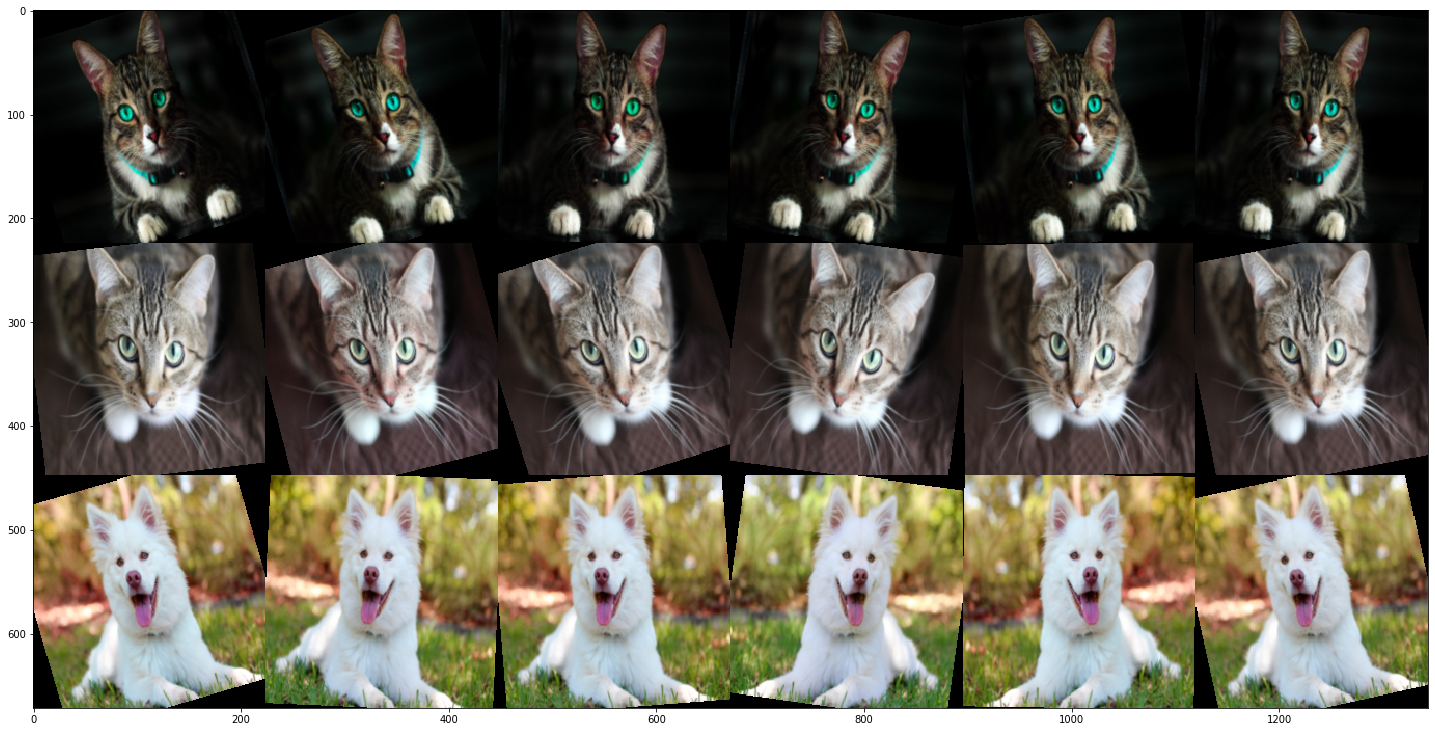
\includegraphics[width=0.9\linewidth]{fig/random_flip_crop_padding.png}
	\caption{Data augmentaion technique based on random flip and crop}
	\label{data_aug}
\end{figure}

\section{Proposed approach}
Our approaches consist of two parts: multilayer perceptron and convolutional neural network.
\subsection{Multilayer perceptron}
We implement multilayer perceptron from scratch. We find that the most difficult parts lie in
\begin{enumerate}[(1)]
	\item How to construct the whole structure of multilayer perceptron
	\item How to back propagate the errors
	\item How to optimize the back propagation to make it not oscillate around the initial values
\end{enumerate}
We will introduce the building mechanism of our work by answering these three questions.

Firstly, in order to give a clear representation of the layer, we define a parent class layer as programming object, which contains the summation vector of $wz+b$, the activation function, loss difference and gradient deviation etc. You can check the code in \texttt{layer.py}. The activation function we use here is ReLU instead of sigmoid, because it is more widely applied. Inherited from basic layer parent class, we define three major layers: \textit{input\_layer}, \textit{hidden\_layer} and \textit{output\_layer}. \textit{input\_layer} and \textit{output\_layer} have slight difference from their parent class, the former does not accept any output and is a container for the input data. As for output layer, we connect it with the last hidden layer and choose \textit{softmax} as its output results. So you can find that output layer has its special attribute \textit{output\_layer.output}. The advantage of defining such class of layers is that we can stack multiple layers when we build the multilayer perceptron, instead of directly defining the weights and bias matrices as many blogs do. You can check in in \textit{MLP.build\_net} in \texttt{mlp.py}.

Secondly, we think the most difficult part in implementing the multilayer perceptron is the back propagation. Let's look at the \textit{MLP.train\_fit}, we flatten the input three-channel figure into one-dimensional vector. After we feed-forward the network to calculate the activations, we firstly compute the back propagation error. By implementing similar code from the slides, we use the one-hot encoding target minus the softmax probability as the output error. And then, we back propagate this error by multiplying weights and derivative of activation functions. If we consider the back propagation procedure in the slides as
\begin{equation*}
	\frac{\partial}{\partial V_{m,d}} = \sum_{c} \frac{\partial L}{\partial \hat{y}_c} \frac{\partial \hat{y}_c}{\partial u_m} \frac{\partial u_m}{\partial z_m} \frac{\partial z_m}{\partial q_m} \frac{\partial q_m}{\partial V_{m,d}}
\end{equation*}
Then \textit{MLP.back\_propgation\_error} computes the 

$$\sum_{c} \frac{\partial L}{\partial \hat{y}_c} \frac{\partial \hat{y}_c}{\partial u_m} \frac{\partial u_m}{\partial z_m} \frac{\partial z_m}{\partial q_m}$$

And then we add \textit{MLP.compute\_gradients\_errors} to make it complete. 

But the back propagation is not yet stable, we therefore add stochastic gradient descent (SGD) with momentum to make the optimization stable in \textit{MLP.compute\_gradients\_errors}. We are confused for a very long time about our accuracy as it is only 0.1 in the beginning, which is only the oscillation around the initialization values. We then realize that it is because the unstable property of SGD. So we add the momentum term for more stable learning with $\beta = 0.9$:

\begin{align*}
	\Delta w^{\{t\}} & \gets \beta \Delta w^{\{t-1\}} + (1-\beta) \nabla J (w^{\{t\}})\\
	w^{\{t\}} & \gets w^{\{t-1\}} - \alpha \Delta w^{\{t\}}
\end{align*}

After update the gradient updates, it would be very easy to implement the rest of the part.

\subsection{Convolutional neural network}
Our implementation of Convolutional neural network is based on the PyTorch documentation example, but we
\begin{enumerate}[(1)]
	\item Use \textit{nn.ModuleList} to make adding any numbers of convolutional layers and fully connected layers possible.
	\item Add comments on each reused code line. 
\end{enumerate}
Because it is reused from the documentation and commented, there is no more details to emphasize.

\section{Results}
\section{Discussion and Conclusion}

\section{Statement for Contributions}
\begin{itemize}
	\item Fuyuan Lyu: 
	\item Tianyu Shi: 
	\item Dingyi Zhuang: 
\end{itemize}
\newpage

\bibliographystyle{unsrt}
\bibliography{ref}

\end{document}
